\paragraph{}Comme dit dans la partie diagramme de classe de l’application client, celui de l’application pour institution financières possède beaucoup de classes ou de concepts en commun avec celle ci.


\begin{figure}[ht]
\centering
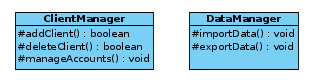
\includegraphics[scale=0.5]{img/ClassBankCommon.png}
\caption{Classes ajoutées dans la partie logique}
\label{fig1}
\end{figure}

\paragraph{Partie logique}La partie banque ajoute 2 classes qui permettent de gérer les clients et les données à savoir ClientManager et DataManager. ClientManager permet grâce à ces méthodes d’ajouter des clients, d’en supprimer ou de gérer leur compte et DataManager permet d’importer des données et d’en exporter.

\paragraph{Partie API} La partie API est exactement la même que l'application client

\newpage

\begin{figure}[ht]
\centering
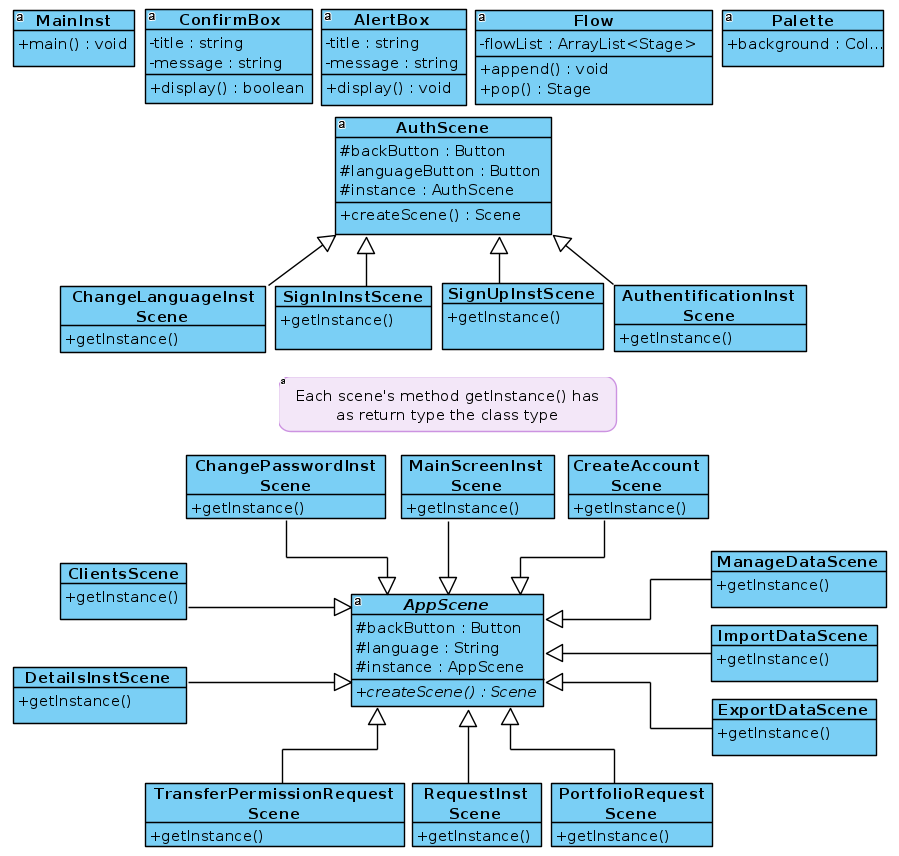
\includegraphics[scale=0.3]{img/GUIBankCommon.png}
\caption{Diagramme de classe de la partie GUI }
\label{fig2}
\end{figure}

\paragraph*{Partie GUI} La partie GUI s’articule de la même manière que celle pour l’application client. On a les classes AuthScene et AppScenes qui sont des classes mères de toutes les autres scenes ainsi que les classes ConfirmBox, AlertBox, Flow et Palette qui sont en commun avec le GUI de la partie client. Le mot clé "Inst" a parfois été ajouté au nom des classes qui ont le même nom que celles de l'application client mais qui ne sont pas les mêmes.
